\section{Semaine 3 : 20/02/2023 - 24/02/2023}
\graphicspath{{semaines/semaine_3/images/}}

\begin{abstract}
	Pour cette semaine, on considère une nouvelle solution analytique (solution trigonométrique : $\sin*\cos$). Avec cette nouvelle solution, on va pouvoir prendre g différent de $u_{ex}$ sur $\Omega$ comme souhaité pendant la semaine précédente. 
	
	A défaut de pouvoir faire tourner les entrainements (car plus d'units dispo sur colab) et en attente d'une solution avec v100, on va s'intéresser uniquement au problème de correction où on prendra comme $\bar{\phi}$ notre $u_{ex}$ ($-g$ si non homogène). En lui donnant comme nouvelle levelset notre solution exacte, $C$ doit être très proche de 1 (à l'erreur machine).  
\end{abstract}

\subsection{Génération des données}

On considère toujours $\Omega$ le cercle de rayon $\sqrt{2}/4$ et de centre $(0.5,0.5)$ avec $\Phi(x,y)=-1/8+(x-1/2)^2+(y-1/2)^2$ et le domaine fictif $O=(0,1)^2$.

On souhaite résoudre 
\begin{equation*}
	\begin{cases}
		-\Delta u &= f\,, \quad \text{dans $\Omega$}\,, \\
		u &= g\,, \quad \text{sur $\Gamma$}\,, \\
	\end{cases}
\end{equation*}

Notre solution analytique est
$$u_{ex}(x,y) = \frac{1}{\sin\left(k_1\frac{\pi}{2}\right)}\times\sin\left(k_1\frac{\pi}{2}\left(\frac{4}{\sqrt{2}}\right)^2\left((x-0.5)^2+(y-0.5)^2\right)\right)\times\cos(k_2(x^2+y^2))\,, $$ 

avec $k_1,k_2 \sim \mathcal{U}([0.1,0.5])$.

Ainsi 
$$g(x,y)=\cos(k_2(x^2+y^2))$$

On considérera également la solution analytique au problème homogène :
$$u_{ex}(x,y) = \frac{1}{\sin\left(k_1\frac{\pi}{2}\right)}\times\sin\left(k_1\frac{\pi}{2}\left(\frac{4}{\sqrt{2}}\right)^2\left((x-0.5)^2+(y-0.5)^2\right)\right)\times\cos\left(\frac{\pi}{2}\left(\frac{4}{\sqrt{2}}\right)^2\left((x-0.5)^2+(y-0.5)^2\right)\right)\,, $$ 

Les formulation faibles sont les mêmes que précédemment.

\subsection{Correction}

Dans un premier temps, on a pris notre nouvel levelset comme étant notre solution exacte sur une image 64*64 puis on interpoler cette levelset (\href{https://colab.research.google.com/drive/15rw2vTlf8yNBIuQPsFHzguUj5fmJiLf9#scrollTo=N2Z4fEjTNpAV}{"u\_trigo\_homogene"}). En prenant $\phi=u_{ex}$, on espère obtenir C très proche de 1 (en augmentant le degré d'interpolation, on espère atteindre l'erreur machine). Les résultats obtenus n'étaient pas bon :

\begin{minipage}{\linewidth}
	\centering
	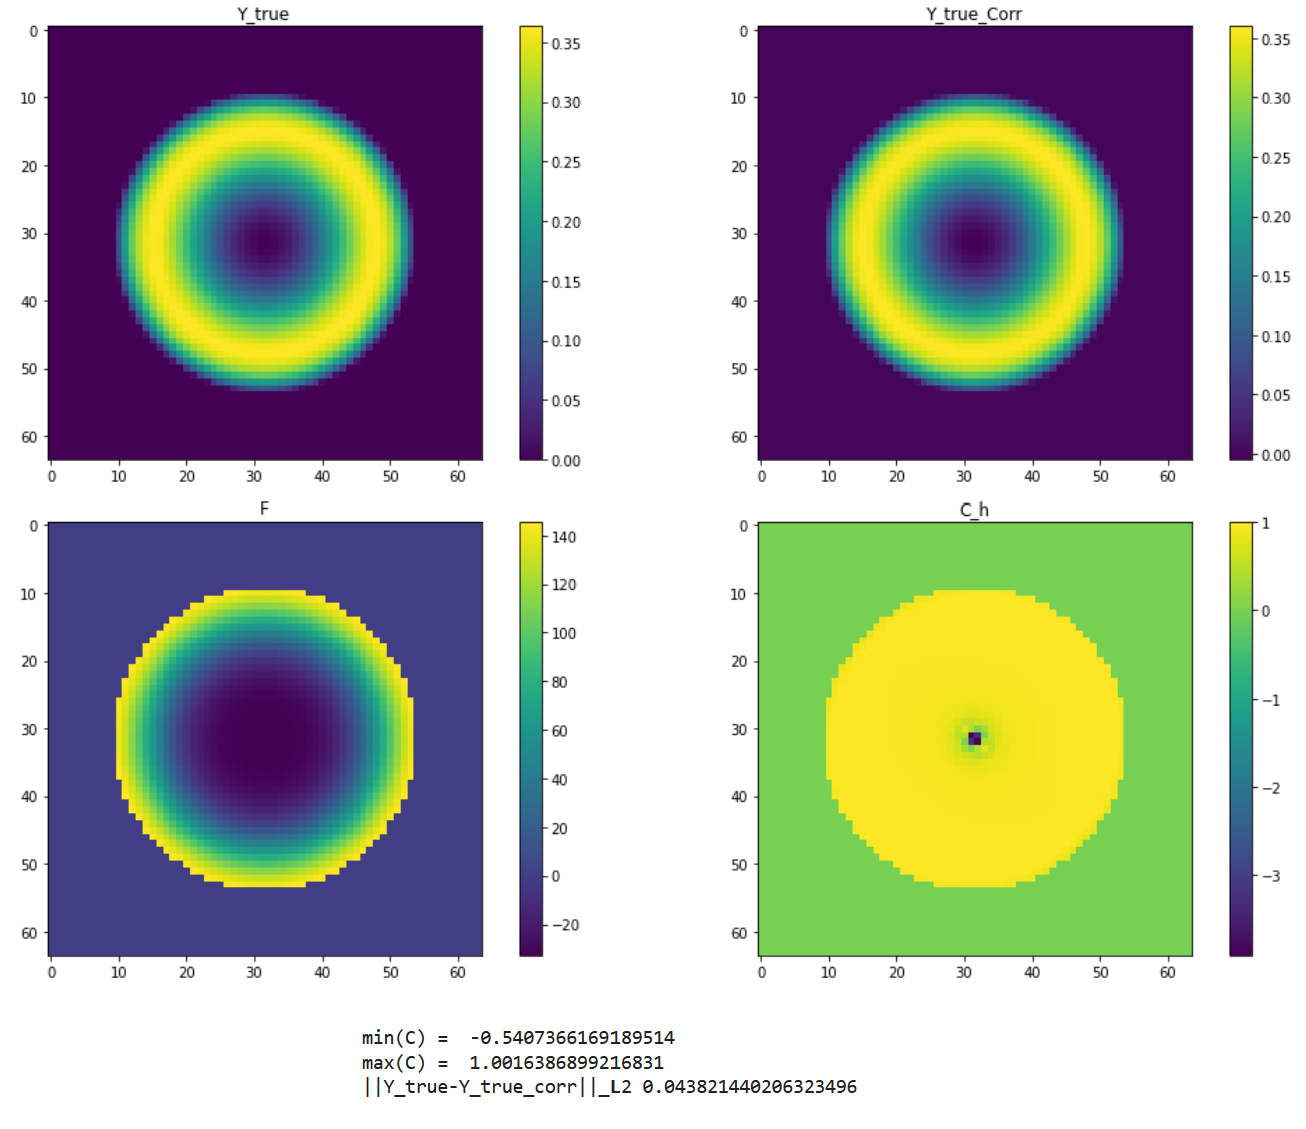
\includegraphics[width=0.45\linewidth]{resultats_correction.png}
\end{minipage}

\newpage 

En fin de semaine, on s'est rendue compte que l'interpolation de $\phi$ posait problème pour la correction. Lorsque $\bar{\phi}=u_{ex}$, on obtient bien l'erreur machine mais en lui donnant notre levelset sous la forme d'une image nb\_vert$\times$nb\_vert (ce qui est plus proche de ce que le réseau fournira), les résultats deviennent incohérents. On a donc tenter deux approches (\href{https://colab.research.google.com/drive/1JOC10OHCCNgTOCPD46bylKhlI1n1_bHR#scrollTo=0w0hQjVlLGwd}{"u\_trigo\_homogene\_modif"}): griddata (de scipy) et extrapolate (de FEniCS). L'option du extrapolate n'a pas fonctionné (nan ?). Pour l'autre option avec le griddata, on a constaté que interpoler avec tous les points de l'image était trop lourd, on a donc décidé de prendre pour chaque point (x,y) un certains nombres de points d'interpolations autour de lui. Voici les résultats obtenus avec différents nb\_vert et différents nombres de points d'interpolation :

\begin{minipage}{\linewidth}
	\centering
	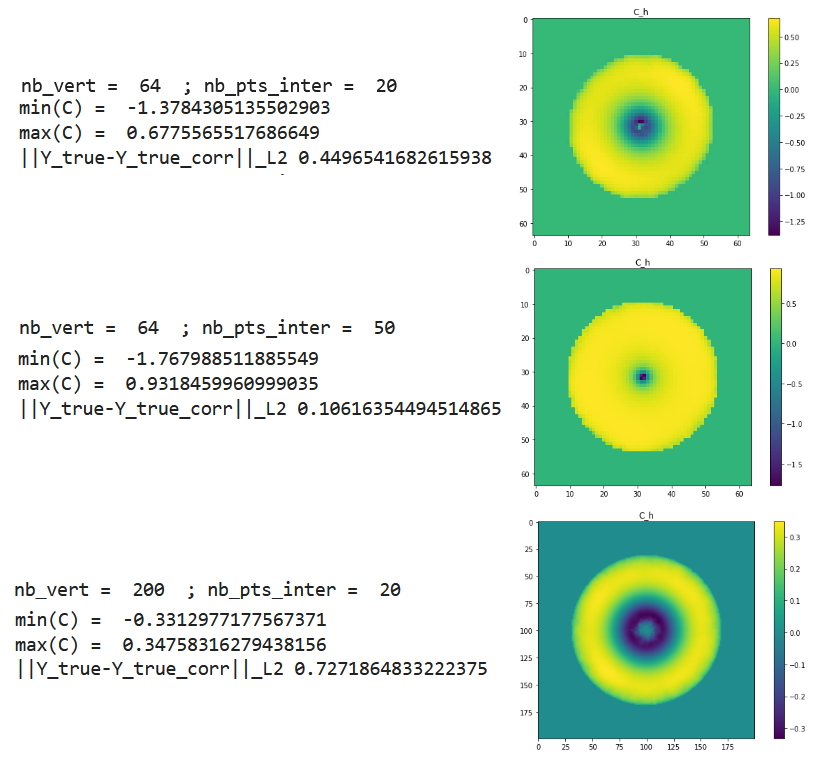
\includegraphics[width=0.6\linewidth]{griddata.png}
\end{minipage}

Ces résultats ont été obtenus la semaine suivante.


\conclusion{L'idée pour la semaine prochaine et d'effectuer quelques tests pour essayer de comprendre ce qui pose problème avec l'interpolation. Une fois ce type de problème réglé, on espère pouvoir entrainer le modèle sur la v100.}